
\documentclass[12pt]{article}

%================= PACKAGES =================
\usepackage[framemethod=default]{mdframed}
\usepackage{graphicx}
\usepackage{tikz}
\usetikzlibrary{decorations.pathreplacing}
\usepackage{float}
\usepackage{amsmath, amssymb}
\usepackage[utf8]{inputenc}
\usepackage[T1]{fontenc}
\usepackage{mathptmx}      % Times New Roman-like text and math
\usepackage{setspace}
\usepackage{booktabs}
\usepackage{caption}
\usepackage[font=small, labelfont=bf]{caption}
\usepackage{microtype}
\usepackage{ntheorem}
\usepackage[hidelinks]{hyperref}
\usepackage[top=2.5cm,bottom=2.5cm,left=2.5cm,right=2.5cm]{geometry}

\theoremseparator{:}
\newtheorem{hyp}{Hypothesis}
\newtheorem{prop}{Proposition}
\newtheorem{thm}{Theorem}

\newcommand{\one}{\mathbf{1}}
\DeclareMathOperator{\cav}{cav}

% simple package-agnostic proof block (avoids amsthm/ntheorem proof clashes)
\newenvironment{pf}{\par\noindent\textit{Proof.}\ \ignorespaces}{\hfill$\square$\par\medskip}

% double spacing as required
\doublespacing

\newenvironment{Definition}[2][]{%
    \begin{mdframed}[
        linewidth=0.5pt,
        backgroundcolor=white,
        skipabove=8pt,
        skipbelow=8pt,
        innertopmargin=6pt,
        innerbottommargin=6pt
    ]
    \ifthenelse{\equal{#2}{}}
        {\textbf{Definition#1.}}
        {\textbf{Definition #1(#2).}}
    \rmfamily\ignorespaces
}{%
    \end{mdframed}%
}
\newenvironment{boxedlemma}[2][]{%
    \begin{mdframed}[
        linewidth=0.5pt,
        backgroundcolor=white,
        skipabove=8pt,
        skipbelow=8pt,
        innertopmargin=6pt,
        innerbottommargin=6pt
    ]
    \ifthenelse{\equal{#2}{}}
        {\textbf{Lemma#1.}}
        {\textbf{Lemma #1#2.}}
    \rmfamily\ignorespaces
}{%
    \end{mdframed}%
}
%-----------------------------------------BEGIN DOC----------------------------------------
\begin{document}

\title{{\Huge \textbf{Research Progress Report}{\large\linebreak\\}}{\Large \textit{Dynamic Bayesian Persuasion}\linebreak\linebreak}}
\author{Hanshuo Ma
\\ \\ \\
\textbf{McMaster University} \\
Department of Economics \\ \\
Instructor: Gajen\\
ECON 701 \\ \\}
\date{July 14, 2026}

\maketitle

\newpage
%-----------------------------------------CONTENT-------------------------------------
\tableofcontents
\newpage

%--------------------------------------Introduction---------------------------------
\section{Introduction}\label{Introduction}

Suppose we live in a world with two states --- Normal and Recession. Households' utility depends on both the state and their own action: they would like to spend in the Normal state and save in a Recession. However, households do not observe which state they are currently in; they can learn about the state's realization only through the central bank's signaling scheme. The central bank's utility, by contrast, is independent of the state: its payoff is tied to the households' action --- specifically, to spending. The central bank observes the evolution of the two-state Markov process and sends messages to households over time in the form of interest-rate guidance. In each period households act on their beliefs about the current state, cutting consumption when they believe a recession is underway and expanding it otherwise, so the bank can keep them spending by signaling a cut. However, the same signal puts households at a disadvantage: signaling a cut also artificially deflates the \textit{exchange rate} in the global market, strengthening the country's exports while making households relatively less wealthy in global terms. To make this concrete, suppose the representative household travels abroad annually on vacation: every artificial cut signal erodes the purchasing power of that trip. If the household knows that the central bank commits fully to its information policy, it will act as the signals direct --- expanding consumption in the Normal state and cutting back in a Recession. But if the household has reason to believe the central bank is only partially committed to its signaling scheme, the signals lose credibility, and the household may prefer to save regardless of what is signaled. A central result of this paper is that this unravelling is not automatic: obedience survives if and only if the degree of commitment clears a threshold, $\lambda_{\mathrm{dyn}}$, characterized below.

\subsection{Motivation}\label{Motivation}

The main distinction of the Bayesian persuasion model that stood out from the traditional models such as cheap talk (Crawford \& Sobel 1982) and signaling games (Spence 1973) is that Bayesian persuasion endows the sender with more commitment power. However, in real life most senders or information designers (i.e.\ an algorithm) are responsible for multiple mandates. For instance, central banks have a dual mandate of minimizing inflation and maximizing employment; the two mandates often require deviation from one another within the context of monetary economics. Hence, the assumption of full commitment needs to be relaxed from time to time, and doing so within a dynamic Bayesian persuasion model rather than a static one-shot canonical model allows us to look into the real-life counterpart with more depth.

The central bank example makes the friction concrete. Modern central banks operate under announced, transparent frameworks --- inflation targets, policy rules, forward guidance --- which are exactly a commitment to an \emph{information policy} in the sense of Kamenica and Gentzkow (2011): the bank announces in advance how its communication will depend on what it observes. What gives the announcement bite is that household spending is belief-driven; what makes it fragile is that the same communication moves the exchange rate. A bank that signals a cut when no recession calls for one deflates the currency and subsidizes exports --- a real temptation delivered by the second mandate, not a modelling device. The commitment embodied in the announced rule is therefore real but imperfect: it is enforced by institutions, reputation, and scrutiny rather than by an unbreakable contract. We capture this with the stochastic-commitment friction of Min (2021): each period the announced rule is honoured with probability $\lambda$, which measures the strength of the institution backing the announcement (Lipnowski, Ravid \& Shishkin 2022). The long-run goal, discussed in Section~\ref{Progress}, is to make $\lambda$ itself an equilibrium object sustained by reputation as in Best \& Quigley (2024), rather than an assumption.

The dynamic setting is equally essential. Business cycles recur: recessions arrive, persist, and end, and the bank must issue guidance again and again over the same cycle. A one-shot persuasion model, or a dynamic model in which the bad state is absorbing, cannot speak to this repetition --- it delivers a single episode of persuasion that ends the first time the truth comes out. Modelling the state as a recurrent Markov chain keeps the persuasion problem alive forever, and, as Section~\ref{Partial} shows, it is precisely the persistence of the recession state (not how often recessions arrive) that determines how much commitment the bank needs.

\subsection{Research question}\label{Research question}

In a dynamic persuasion model with exogenous partial commitment and a recurrent Markov process, what is the optimal policy? Is it delaying disclosure while risk is low and then revealing a state change only as often as obedience requires?

\subsection{Approach}\label{Approach}

The main model follows the dynamic Bayesian persuasion literature (Ely 2017) closely apart from a few important distinctions. Instead of two states where one is absorbing, in this paper no state is absorbing. Therefore, good behaviour is no longer front-loaded: the agent no longer changes behavior exactly once, from working to shirking. The partial commitment set-up follows Min (2021): the announced signal is honoured with probability $\lambda$; with probability $1-\lambda$ the bank re-optimises (cheats).

\subsection{Related literature and contribution}\label{Literature}

The canonical static model of Kamenica and Gentzkow (2011) consists of one sender and one receiver. The receiver must take an action, and the receiver's utility from that action is state-dependent; the sender's utility is state-independent, depending only on the action the receiver takes (as in their leading example, and as in this paper). The sender's goal is to design an information policy that persuades the receiver into the sender-preferred action as often as possible, regardless of which state is realized. The defining assumption is commitment: the sender commits to a signaling scheme before the state realizes, and the scheme is fixed and publicly known to the receiver. Upon observing the signal realization, the receiver updates beliefs via Bayes' rule. The induced distribution of posteriors must satisfy Bayes plausibility: it must average back to the prior belief. The optimal scheme is then read off a concavification: writing the sender's payoff as a function of the receiver's posterior, the sender's value is the concave envelope of that function evaluated at the prior, and the optimal signal splits the prior into the posteriors that support the envelope.

This project sits at the intersection of two strands that have, so far, mostly been studied separately, each relaxing the canonical model in one direction.

The first strand is \emph{dynamic} persuasion with full commitment. Ely (2017) is the backbone: a principal observes an evolving state and commits to a disclosure policy, and the value function is characterized recursively as the concave envelope of the flow payoff plus the discounted continuation value, $V=\cav[(1-\delta)u+\delta(V\circ f)]$. In Ely's leading model, however, the bad state is \emph{absorbing}: the belief drifts monotonically toward certainty, the optimal ``beep'' is a one-time delayed disclosure, and once the truth is out the game is effectively over ($V(1)=0$). The second strand relaxes commitment in \emph{static} persuasion: Min (2021) has the sender's announced signal honoured only with probability $\lambda$, Lipnowski, Ravid and Shishkin (2022) interpret $\lambda$ as the strength of a weak institution, and Best and Quigley (2024) ask when repeated interaction and reputation can substitute for commitment in the long run.

Two recent contributions mark the boundaries of this relaxation exercise, and clarify where the sender's power comes from. Arieli and Stewart (2025) remove commitment entirely but make disclosure \emph{verifiable} --- the sender can conceal evidence but cannot fabricate it --- and show that under general conditions the sender nevertheless attains the full-commitment persuasion payoff: verifiability substitutes for commitment. Danilov and Lambert-Mogiliansky (2018a,b) relax a different assumption of Kamenica and Gentzkow (2011) altogether, namely the receiver's classical Bayesian cognition: when beliefs are quantum-like states and messages act as non-commuting \emph{measurements}, the martingale property of posteriors fails, and a suitable sequence of measurements can induce essentially \emph{any} belief --- with limited opportunities, a targeted belief is reached with probability at least $1/n$ (Danilov and Lambert-Mogiliansky 2018a). The comparison is instructive: for a Bayesian receiver, Bayes plausibility caps manipulation \emph{regardless of commitment} --- posteriors must average back to the prior, so the receiver can always fall back on ignoring uninformative messages, which is why weakening commitment can only (weakly) hurt the sender (Min 2021) --- whereas relaxing Bayesian updating removes the cap entirely. This project stays within the Bayesian, unverifiable-message direction, the empirically relevant one for central-bank guidance addressed to markets that update consistently.

The contribution of this project is to combine the two strands, with one further change that does real work: the state follows a \emph{recurrent} Markov chain rather than Ely's absorbing one. This generalization matters for three reasons. First, it is the empirically relevant case for the macroeconomic application --- business cycles recur, so guidance is a stationary, repeated problem rather than a single episode; the absorbing model is nested as the limit $b \to 0$ of ours (Section~\ref{Solving}). Second, recurrence changes the structure of the solution: certainty is no longer terminal ($V(1)>0$), Ely's terminal condition disappears and both boundary values of the value function become genuine unknowns, and the one-time delayed beep becomes a stationary \emph{delay-then-ration cycle} (Proposition~\ref{prop:optfc}). Third --- and this is where the two strands interact --- recurrence is exactly what makes partial commitment analytically tractable and economically interesting: because disclosure must be delivered again and again along the cycle, credibility becomes a \emph{per-period} constraint, and it collapses into a single sufficient statistic $\lambda_{\mathrm{dyn}}$ that depends on the persistence of the recession state but not on its arrival rate (Propositions~\ref{prop:lambda} and~\ref{prop:speed}). In the absorbing model this question is degenerate: there is only one disclosure event to be tempted about.

The combination also raises further research questions that neither strand faces alone, developed in Section~\ref{Progress}: what disclosure is optimal when the institution is too weak ($\lambda<\lambda_{\mathrm{dyn}}$); whether $\lambda$ can be endogenized as a reputation state in the spirit of Best and Quigley (2024) but in a recurrent environment where the sender is tempted infinitely often; and how the welfare accounting changes once the exchange-rate externality that motivates cheating enters the payoff explicitly.

%--------------------------------------Model---------------------------------
\section{One-Sender, One-Receiver Model in Discrete Time}\label{Model}

Suppose that the agent has a threshold $p^*$ such that she will start saving as soon as she believes with probability greater than $p^*$ that a recession is happening. The agent enters period $t$ with belief $\mu_t$. The principal then observes the current state $s_t$, draws their own commitment type and sends a message to the agent accordingly. In response to the message the agent updates to an interim belief $\nu_t$ and takes an action. All of the preceding can be regarded as happening instantaneously. Next, a discrete length of time passes and we enter period $t+1$.

The agent's choice of action $a_t$ maximizes the expected value of her state-dependent utility function $x$, $a_t \in \arg\max_a \mathbb{E}_{\nu_t} x(a,s)$. The principal's payoff $u(a,s)$ indirectly depends on the agent's interim belief, i.e., $u(\nu,s) = u(a(\nu),s)$. The long-run average discounted payoff of the principal is then $(1-\delta)\sum_{t=0}^{\infty}\delta^t u(\nu_t, s_t)$, where $\delta \in (0,1)$ is the discrete-time discount factor.

A policy for the principal is a rule $\sigma(h_t) \in \Delta M_t$ which maps the principal's complete prior history $h_t$ into a probability distribution over messages, where the message space $M_t$ is unrestricted.

\paragraph{Messages as interest-rate guidance.} The message space is left unrestricted --- the obfuscation principle below handles arbitrary message spaces, and no reduction is imposed. On the path of the optimal policy, however, only two messages are ever used, and we name them by the instrument they represent: \textsc{cut}, the reassuring guidance that keeps the household spending, and \textsc{raise}, an increase in the policy rate, which is the disclosure event (the ``beep'' of Ely 2017). The \textsc{raise} is not a withholding of speech but an \emph{informative signal}: on the optimal path it is issued only in the recession state, so it reveals the state outright. A period in which the announced rule issues \textsc{cut} in both states with probability one is \emph{uninformative}: the guidance is uncorrelated with the state and beliefs move by drift alone. We avoid Ely's term ``silence'' altogether --- the bank always speaks; what varies over the cycle is whether its guidance carries information. Two messages, two regimes: \emph{uninformative} thus describes a period's announced rule, never a third message. Indeed, the same \textsc{cut} message that carries no information in the delay phase becomes informative in the rationing phase of Section~\ref{Policy}, where it is good news: conditional on \textsc{cut}, the posterior returns to exactly $p^*$ (equation \eqref{eq:rhostar}).

The principal's flow payoff therefore reduces to a function of the interim belief alone. Writing beliefs as the probability assigned to the recession state, the flow payoff is
\[
u(\nu)=
\begin{cases}
1 & \nu \le p^* \\
0 & \nu > p^*
\end{cases}
\]

\noindent\emph{Notation.} Throughout, $\mu_t$ denotes the belief entering period $t$ and $\nu_t$ the interim belief after the period-$t$ message, so that $\mu_{t+1}=f(\nu_t)$; under uninformative guidance $\nu_t=\mu_t$. When no timing is at stake --- as in the arguments of the functions $u$, $V$, $f$, and $\rho^*$ below --- a generic belief is written $\mu\in[0,1]$.

\noindent\emph{Remark (who computes the belief).} The belief $\mu_t$ is public: it is pinned down by the common prior $\mu_0$, the announced rule, and the history of messages, all of which both parties observe. The bank therefore does not \emph{observe} the household's belief --- it \emph{computes} it, replicating the household's Bayes step to obtain $\nu_t$ and then applying the drift $\mu_{t+1}=f(\nu_t)$. For the same reason, the three phases of the optimal policy in Section~\ref{Policy} are not three separate commitments: the bank commits once, at time zero, to a single state- and belief-contingent rule, and the phases are simply the regions of $[0,1]$ that the computable belief path visits. Along the delay phase the belief follows a deterministic drift in closed form, so the bank knows already at time zero the calendar period at which disclosure must begin. Under partial commitment (Section~\ref{Partial}) the household's computation replaces the promised disclosure rate $\rho$ by the effective rate $\lambda\rho$; since $\lambda$ is common knowledge, the belief remains a public state variable. All of this relies on the assumption, stated in the Introduction, that households learn about the state only through the bank's guidance; if households also observed an exogenous public or private signal, the belief would become a stochastic state that the bank tracks with error --- a natural extension beyond this report.

In this basic model, there are two states $s_t \in S = \{N,R\}$, and the agent has two actions $a \in \{0,1\}$. The process is a recurrent two-state Markov chain with the following transition matrix:
\[
P=\begin{pmatrix}1-a & a\\[2pt] b & 1-b\end{pmatrix}
\]
$a=\Pr(s_{t+1}=R \mid s_t = N)$, $b=\Pr(s_{t+1}=N \mid s_t = R)$, where $a,b\in(0,1)$, $a>b$, $a+b<1$. The set-up here is to make the recession state ($R$) more ``sticky'' in the stationary distribution $\mu^*$. Solving $\pi P = \pi$ with $\pi_N + \pi_R = 1$ gives $\pi_N a = \pi_R b$, hence
\[
\mu^* = (\pi_N, \pi_R) = \Big(\frac{b}{a+b},\ \frac{a}{a+b}\Big) = (1-\mu_R^*,\ \mu_R^*),
\qquad \mu_R^* = \frac{a}{a+b} .
\]
Because $a>b$ we have $\mu_R^* > \tfrac12$: the recession state is entered faster than it is left, so beliefs rest above one half.

Here we are more interested in the case where $\mu_R^* > p^*$: in the long run, if the stationary belief satisfied $\mu_R^* \le p^*$, the principal would simply leave the agent be and let them keep spending forever. Under this non-degeneracy condition, the interval $I=(p^*,1]$ is an absorbing interval under the belief map $f$ defined below, and the flow payoff $u \equiv 0$ is (trivially) linear on $I$; therefore, using Lemma 1 from Ely (2017, Online Appendix 6.2), the value function $V$ must be affine on $I$.

\begin{boxedlemma}{ 1 From Ely (2017 Online Appendix 6.2)}
Suppose that $I$ is absorbing under $f$, and that $u$ is linear over $I$. Then $V$ is also linear on $I$. Here $V$ is the value function of the dynamic problem: it is the concavification of a function that involves the value function itself, extending the static persuasion of Kamenica and Gentzkow (2011).
\end{boxedlemma}

\begin{Definition}{Belief map}
The Markov chain induces a belief-transition map $f:\Delta(\Theta)\to\Delta(\Theta)$. If today's belief is $\mu$ then the receiver's belief at the start of next period is the one-step prediction $f(\mu) = P^{\top}\mu$.
\end{Definition}
\[
P^{\top}\mu=
\begin{pmatrix}1-a & b\\ a & 1-b\end{pmatrix}
\begin{pmatrix}\mu_N\\ \mu_R\end{pmatrix}
=\begin{pmatrix}(1-a)\mu_N + b\,\mu_R\\[4pt] a\,\mu_N + (1-b)\,\mu_R\end{pmatrix}.
\]
Taking the $R$-component and substituting $\mu_N = 1-\mu_R = 1-\mu$:
\begin{align*}
a(1-\mu)+(1-b)\mu &= a - a\mu + \mu - b\mu\\
&= a + \mu\,(1-a-b)\\
&= a + (1-a-b)\,\mu = f(\mu).
\end{align*}

\noindent\emph{Remark (the discarded $N$-component and the geometry of the simplex).} Tracking only the $R$-component is without loss. Each row of $P$ sums to one, hence each column of $P^{\top}$ sums to one, so the entries of $P^{\top}\mu$ automatically sum to $\mu_N+\mu_R=1$: the belief map sends the simplex to itself. The $N$-component is therefore exactly the complement,
\[
(1-a)(1-\mu)+b\mu = (1-a)-(1-a-b)\mu = 1-f(\mu),
\]
and carries no independent information. Since a belief over two states has a single degree of freedom, the simplex $\Delta(\{N,R\})=\{(\mu_N,\mu_R)\in\mathbb{R}^2_+:\mu_N+\mu_R=1\}$ is one-dimensional --- the line segment joining the degenerate beliefs $e_N=(1,0)$ and $e_R=(0,1)$ --- and we identify it with $[0,1]$ via $\mu=\mu_R$ (Figure~\ref{fig:simplex}). Under this identification the vertex $e_R$, certainty of recession, is the point $\mu=1$, referred to below as the \emph{top} of the simplex. This reduction is what makes the concavification below literal one-dimensional geometry --- chords on an interval and a kink at $p^*$, drawn in Figure~\ref{fig:geometry} --- and it is special to two states: with $n$ states the simplex is $(n-1)$-dimensional and the concave envelope must be found over a multi-dimensional domain. As a consistency check, the fixed point of the discarded component is $1-\mu_R^* = b/(a+b)$, the stationary mass on $N$: the two components of $P^{\top}\mu$ are just the two coordinates of the stationary distribution at rest.

\begin{figure}[H]
\centering
\begin{tikzpicture}[scale=3.6, font=\scriptsize]
% ---- left: the simplex as a segment in R^2 ----
\draw[->] (0,0) -- (1.2,0) node[right] {$\mu_N$};
\draw[->] (0,0) -- (0,1.2) node[left] {$\mu_R$};
\draw[very thick] (1,0) -- (0,1);
\fill (1,0) circle (0.014);
\fill (0,1) circle (0.014);
\node[below] at (1,-0.03) {$e_N=(1,0)$};
\node[left] at (-0.03,1) {$e_R=(0,1)$};
\node[above right] at (0.52,0.52) {$\Delta(\{N,R\})$};
% generic belief
\fill[blue!55!black] (0.2,0.8) circle (0.014);
\node[above right, blue!55!black] at (0.20,0.80) {$(1-\mu,\ \mu)$};
\draw[dashed] (0.2,0.8) -- (0.2,0) node[below] {$1-\mu$};
\draw[dashed] (0.2,0.8) -- (0,0.8) node[left] {$\mu$};
% ---- identification arrow ----
\draw[->, thick] (1.32,0.5) -- (1.62,0.5) node[midway, above] {$\mu=\mu_R$};
% ---- right: the interval [0,1] ----
\draw[very thick] (1.8,0.5) -- (2.8,0.5);
\fill (1.8,0.5) circle (0.014);
\fill (2.8,0.5) circle (0.014);
\fill[blue!55!black] (2.6,0.5) circle (0.014);
\draw (2.3,0.485) -- (2.3,0.515);
\node[below] at (1.8,0.47) {$0$};
\node[below] at (2.3,0.47) {$p^*$};
\node[below] at (2.6,0.47) {$\mu$};
\node[below] at (2.8,0.47) {$1$};
\node[above, align=center] at (1.8,0.55) {certainty\\of $N$};
\node[above, align=center] at (2.8,0.55) {certainty of $R$\\(``top'')};
\end{tikzpicture}
\caption{The belief simplex for two states. \emph{Left:} $\Delta(\{N,R\})$ is the line segment $\{(\mu_N,\mu_R)\in\mathbb{R}^2_+:\mu_N+\mu_R=1\}$; its vertices are the degenerate beliefs, and a generic belief $(1-\mu,\mu)$ sits between them. \emph{Right:} identifying each belief with its $R$-coordinate maps the segment onto $[0,1]$. The ``top of the simplex'' is the vertex $\mu=1$ (all mass on $R$) --- the point where the recurrent model has $V(1)>0$ while the absorbing model has $V(1)=0$.}
\label{fig:simplex}
\end{figure}

The map $f$ is affine with slope $1-a-b \in (0,1)$, and its unique fixed point solves $\mu = a+(1-a-b)\mu$, i.e.\ $\mu = \tfrac{a}{a+b} = \mu_R^*$: the deterministic belief drift and the stochastic chain share the same rest point, which confirms the stationary distribution above. To verify the absorbing-interval claim: $f(p^*)-p^* = a-(a+b)p^* = (a+b)(\mu_R^*-p^*) > 0$ and $f(1) = 1-b < 1$, so $f$ maps $(p^*,1]$ into itself.

\noindent\emph{Remark (the four roles of the belief map).} Since the household acts on beliefs rather than on states --- it never observes $s_t$ --- the state process leaves its trace on the model only through $f$: the entire two-state chain $P$ is compressed into this one affine map on the one-dimensional simplex (Figure~\ref{fig:simplexmap}), its slope $1-a-b$ the chain's persistence and its fixed point the stationary distribution. It is worth listing at the outset the four distinct places where $f$ does its work in what follows. \emph{(i) $f$ is the clock.} Under uninformative guidance $\nu_t=\mu_t$, so the belief drifts deterministically along $f$ toward $\mu_R^*$; starting below the threshold, the drift \eqref{eq:drift} crosses $p^*$ at the hitting time \eqref{eq:hit}, which fixes the length of the delay phase of the optimal policy (Section~\ref{Policy}). \emph{(ii) $f$ links the periods.} In the recursion \eqref{eq:cav} the future enters only through the composition $V\circ f$; without it the dynamic problem would collapse into a sequence of static concavifications. \emph{(iii) $f$ at the threshold forces disclosure.} Because $\varphi = f(p^*)>p^*$ (just computed), guidance that carries no information pushes the belief past the threshold into the no-spending region, so holding the household at $p^*$ requires the informative \textsc{raise} to be rationed at exactly the rate $\rho^*$ in \eqref{eq:rhostar}. \emph{(iv) $f$ at the top delivers recurrence and the credibility bound.} $f(1)=1-b<1$: certainty is not a fixed point of the belief map, so a \textsc{raise} is non-terminal and $V(1)>0$ (Section~\ref{Solving}); the same number $1-b$ is then the largest on-path belief at which rationing operates, so the commitment threshold of Section~\ref{Partial} is $\lambda_{\mathrm{dyn}} = \rho^*(1-b)$, and Theorem~\ref{thm:equiv} records $f(1)<1$ as the belief-dynamics expression of recurrence, equivalent to the primitive $b>0$, ergodicity of $P$, $V(1)>0$, and $\lambda_{\mathrm{dyn}}<1$. A final consequence of $f$ being deterministic and affine: the on-path rationing beliefs form the finite cycle $\{\varphi,\,1-b\}$, which is what reduces the one-shot-deviation check of Section~\ref{Progress} to a small linear system.

\begin{figure}[H]
\centering
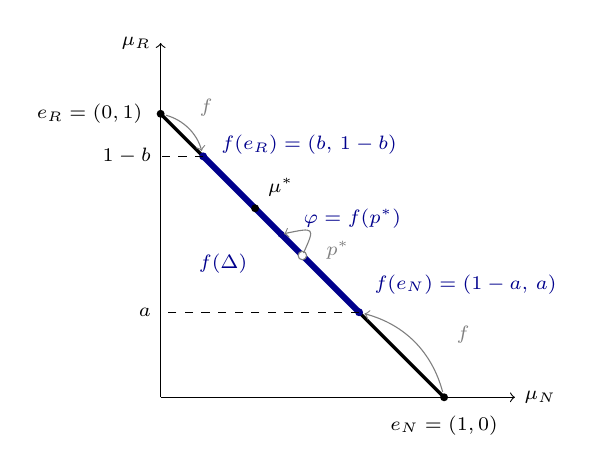
\begin{tikzpicture}[scale=3.6, font=\scriptsize]
% axes
\draw[->] (0,0) -- (1.25,0) node[right] {$\mu_N$};
\draw[->] (0,0) -- (0,1.25) node[left] {$\mu_R$};
% the simplex
\draw[very thick] (1,0) -- (0,1);
% the image segment f(Delta), a strict sub-segment of the simplex
\draw[line width=2.2pt, blue!55!black] (0.7,0.3) -- (0.15,0.85);
\node[blue!55!black, anchor=east] at (0.34,0.47) {$f(\Delta)$};
% vertices
\fill (1,0) circle (0.014);
\node[below] at (1,-0.03) {$e_N=(1,0)$};
\fill (0,1) circle (0.014);
\node[left] at (-0.03,1) {$e_R=(0,1)$};
% images of the vertices
\fill[blue!55!black] (0.7,0.3) circle (0.014);
\node[blue!55!black, anchor=south west] at (0.72,0.33) {$f(e_N)=(1-a,\,a)$};
\fill[blue!55!black] (0.15,0.85) circle (0.014);
\node[blue!55!black, anchor=west] at (0.18,0.89) {$f(e_R)=(b,\,1-b)$};
% threshold and its image
\draw[gray, fill=white] (0.5,0.5) circle (0.015);
\node[gray, anchor=west] at (0.55,0.52) {$p^*$};
\fill[blue!55!black] (0.425,0.575) circle (0.012);
\node[blue!55!black, anchor=west] at (0.47,0.63) {$\varphi=f(p^*)$};
% fixed point (stationary distribution)
\fill (0.3333,0.6667) circle (0.014);
\node[anchor=south west] at (0.345,0.675) {$\mu^*$};
% arrows of the map
\draw[->, gray, shorten >=2pt, shorten <=2pt] (1,0) to[bend right=30] (0.7,0.3);
\node[gray, anchor=west] at (1.01,0.22) {$f$};
\draw[->, gray, shorten >=2pt, shorten <=2pt] (0,1) to[bend left=30] (0.15,0.85);
\node[gray] at (0.16,1.02) {$f$};
\draw[->, gray, shorten >=1pt, shorten <=1pt] (0.5,0.5) .. controls (0.545,0.60) .. (0.425,0.575);
% guides: the image interval [a, 1-b] on the R-axis
\draw[dashed] (0.15,0.85) -- (0,0.85) node[left] {$1-b$};
\draw[dashed] (0.7,0.3) -- (0,0.3) node[left] {$a$};
\end{tikzpicture}
\caption{The belief map acting on the simplex, drawn to scale for the same parameters as Figure~\ref{fig:geometry} ($a=0.3$, $b=0.15$, $p^*=0.5$). The affine map $f(\mu)=P^{\top}\mu$ sends the simplex into itself, and its image $f(\Delta)$ (thick blue) is the strict sub-segment with $R$-coordinate in $[a,\,1-b]$: one step of drift wipes out certainty of either state. The three grey arrows are the three motions that drive the paper. The vertex $e_N$ jumps to $(1-a,a)$: even a household certain of Normal expects recession risk $a$ tomorrow, which starts the Phase~A drift. The threshold $p^*$ is pushed past itself to $\varphi=f(p^*)$, which is what forces the rationing of informative \textsc{raise}s (Section~\ref{Policy}). The top vertex $e_R$ is pulled down to $(b,1-b)$ --- the geometric form of $f(1)=1-b<1$, item (ii) of Theorem~\ref{thm:equiv}. The unique point that stays put is the fixed point $\mu^*$, the stationary distribution. In the absorbing benchmark $b=0$ the blue segment would reach the top vertex and $f(e_R)=e_R$: certainty of recession would be a trap, and with it $V(1)=0$.}
\label{fig:simplexmap}
\end{figure}

\begin{figure}[H]
\centering
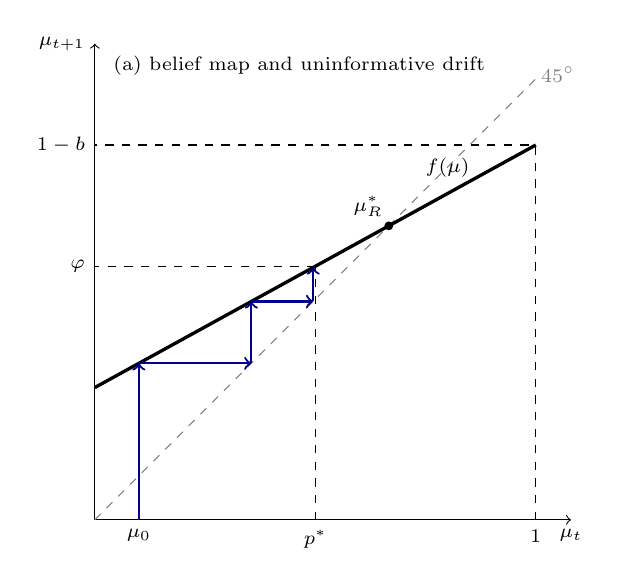
\begin{tikzpicture}[scale=5.6, font=\scriptsize]
% ---------- Panel (a): belief map on the 1-D simplex ----------
\draw[->] (0,0) -- (1.08,0) node[below] {$\mu_t$};
\draw[->] (0,0) -- (0,1.08) node[left] {$\mu_{t+1}$};
\draw[dashed, gray] (0,0) -- (1,1);
\node[gray, right] at (0.99,1.01) {$45^\circ$};
\draw[very thick] (0,0.3) -- (1,0.85);
\node[above, sloped] at (0.80,0.755) {$f(\mu)$};
\fill (0.6667,0.6667) circle (0.010);
\node[above left] at (0.675,0.665) {$\mu_R^*$};
% cobweb from mu0 = 0.1
\draw[->, thick, blue!55!black] (0.1,0) -- (0.1,0.355);
\draw[->, thick, blue!55!black] (0.1,0.355) -- (0.355,0.355);
\draw[->, thick, blue!55!black] (0.355,0.355) -- (0.355,0.4953);
\draw[->, thick, blue!55!black] (0.355,0.4953) -- (0.4953,0.4953);
\draw[->, thick, blue!55!black] (0.4953,0.4953) -- (0.4953,0.5724);
\node[below] at (0.1,0) {$\mu_0$};
% threshold and images
\draw[dashed] (0.5,0) node[below] {$p^*$} -- (0.5,0.575);
\draw[dashed] (0.5,0.575) -- (0,0.575) node[left] {$\varphi$};
\draw[dashed] (1,0) node[below] {$1$} -- (1,0.85) -- (0,0.85) node[left] {$1-b$};
\node[anchor=west] at (0.02,1.03) {(a) belief map and uninformative drift};
\end{tikzpicture}
\hfill
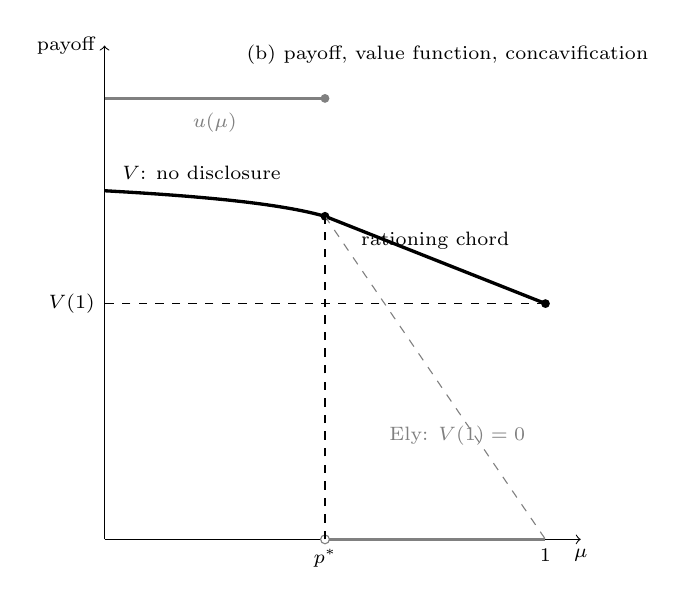
\begin{tikzpicture}[scale=5.6, font=\scriptsize]
% ---------- Panel (b): payoff, value function, concavification ----------
\draw[->] (0,0) -- (1.08,0) node[below] {$\mu$};
\draw[->] (0,0) -- (0,1.12) node[left] {payoff};
% step payoff u
\draw[very thick, gray] (0,1) -- (0.5,1);
\fill[gray] (0.5,1) circle (0.010);
\draw[very thick, gray] (0.5,0.0) -- (1,0.0);
\draw[gray, fill=white] (0.5,0.0) circle (0.010);
\node[gray, below] at (0.25,0.99) {$u(\mu)$};
% V: no-disclosure region (from closed form), then rationing chord
\draw[very thick, domain=0:0.5, smooth, samples=30]
  plot (\x, {1-0.2673*exp(0.17626*ln(0.16667/(0.66667-\x)))});
\draw[very thick] (0.5,0.7327) -- (1,0.5347);
\fill (0.5,0.7327) circle (0.010);
\fill (1,0.5347) circle (0.010);
\node[above] at (0.22,0.795) {$V$: no disclosure};
\node[above, sloped] at (0.75,0.635) {rationing chord};
% Ely's absorbing benchmark for contrast
\draw[dashed, gray] (0.5,0.7327) -- (1,0);
\node[below, sloped, gray] at (0.80,0.28) {Ely: $V(1)=0$};
% guides
\draw[dashed] (0.5,0) -- (0.5,0.7327);
\node[below] at (0.5,0) {$p^*$};
\draw[dashed] (1,0.5347) -- (0,0.5347) node[left] {$V(1)$};
\node[below] at (1,0) {$1$};
\node[anchor=west] at (0.30,1.10) {(b) payoff, value function, concavification};
\end{tikzpicture}
\caption{The geometry of the solution on the one-dimensional simplex. \emph{Panel (a):} the affine belief map $f(\mu)=a+(1-a-b)\mu$, its fixed point $\mu_R^*$ (also the stationary recession probability), and the uninformative-guidance drift from $\mu_0$ cobwebbing up to the threshold $p^*$; the images $\varphi=f(p^*)$ and $1-b=f(1)$ bound the absorbing interval. \emph{Panel (b):} the step flow payoff $u$ (grey), the concave value function $V$ on the no-disclosure region $[0,p^*]$, and the affine rationing chord joining $(p^*,V(p^*))$ to $(1,V(1))$ --- the kink at $p^*$ is where disclosure begins. The dashed grey chord is Ely's absorbing benchmark, where $V(1)=0$; the vertical gap at $\mu=1$ is the recurrence premium. Drawn to scale for $a=0.3$, $b=0.15$, $p^*=0.5$, $\delta=0.9$ using the closed forms of Section~\ref{Solving}: $V(p^*)=0.733$, $V(1)=0.535$.}
\label{fig:geometry}
\end{figure}

%--------------------------------------Full commitment---------------------------------
\section{Full-commitment benchmark}\label{FullCommitment}

Before relaxing commitment we solve the principal's problem under full commitment, which both fixes the benchmark payoff and pins down the optimal disclosure policy that partial commitment must later sustain, as shown in Min (2021).

\subsection{The Bellman equation}\label{Bellman}

Now in order to obtain the value function, we need the Obfuscation Principle from Ely (2017) to fully characterize the dynamic optimization problem.

\begin{boxedlemma}{ 2 (The Obfuscation Principle)}
Any policy $\sigma$ induces a stochastic process $(\mu_t, \nu_t)$ satisfying
\begin{enumerate}
\item $\mathbb{E}(\nu_t \mid \mu_t) = \mu_t$
\item There exists a linear map $f$ s.t.\ $\mu_{t+1} = f(\nu_t)$
\end{enumerate}
\end{boxedlemma}

The principal's expected payoff from such a policy is
\[
\mathbb{E}\sum_{t=0}^{\infty}\delta^t u(\nu_t)
\]

With Lemma 2, we can state our Bellman equation:
\begin{align}
V(\mu_t) &= \max_{q\in\Delta(\Delta S),\ \mathbb{E}q=\mu_t} \mathbb{E}_q\big[(1-\delta)u(\nu_t) + \delta(V\circ f)(\nu_t)\big] \label{eq:bellman}\\
V &= \cav\big[(1-\delta)u + \delta(V\circ f)\big] \label{eq:cav}
\end{align}

Here $\cav$ denotes concavification as in Kamenica and Gentzkow (2011). However, in contrast to the static persuasion problem, the difficulty is that the value function being concavified here appears on both sides of the equation. Thus, going back to Lemma 1: since we have already shown that the interval $I=(p^*,1]$ is absorbing and $u$ is linear there, the value function $V$ is affine on $I$. Restricting attention to the region $I$, the real-valued affine function $V(\mu) = \vec{a}\mu + \vec{b}$ on $(p^*,1]$ is completely determined by its values at exactly two points, $V(p^*)$ and $V(1)$:
\begin{align}
V(p^*) &= \vec{a}p^* + \vec{b} \label{eq:atpstar}\\
V(1) &= \vec{a} + \vec{b} \label{eq:atone}\\
V(1)-V(p^*) &= \vec{a}(1-p^*) \nonumber\\
\vec{a} &= \frac{V(1)-V(p^*)}{1-p^*} \label{eq:slope}
\end{align}
Now once we have $\vec{a}$, we can plug this back in equation \eqref{eq:atone} and solve for $\vec{b}$:
\begin{align}
\vec{b} &= V(1) - \vec{a} \nonumber\\
\vec{b} &= V(1) - \frac{V(1)-V(p^*)}{1-p^*} \nonumber\\
\vec{b} &= \frac{V(p^*) - p^*V(1)}{1-p^*} \label{eq:intercept}
\end{align}
Finally, the affine function $V(\mu) = \vec{a}\mu + \vec{b}$ has the form:
\begin{equation}\label{eq:chord}
V(\mu) = \frac{V(1)-V(p^*)}{1-p^*}\,\mu + \frac{V(p^*)-V(1)p^*}{1-p^*}
\qquad \forall\,\mu\in[p^*,1]
\end{equation}
It is convenient to record an equivalent form of \eqref{eq:chord}. On $[p^*,1]$ the graph of $V$ is the \emph{chord} joining $(p^*,V(p^*))$ and $(1,V(1))$ --- chord being the standard convex-analysis term for the line segment connecting two points on a graph, as in the definition of a concave function as one lying above its chords. Collecting the $V(p^*)$ and $V(1)$ terms in \eqref{eq:chord} and defining the weight
\begin{equation}\label{eq:weight}
w(\mu) := \frac{\mu-p^*}{1-p^*},
\qquad\text{so that}\qquad
1-w(\mu) = \frac{1-\mu}{1-p^*},
\end{equation}
the chord form reads
\begin{equation}\label{eq:chord2}
V(\mu) = \frac{(1-\mu)\,V(p^*) + (\mu-p^*)\,V(1)}{1-p^*}
= \big(1-w(\mu)\big)\,V(p^*) + w(\mu)\,V(1),
\qquad \mu\in[p^*,1].
\end{equation}
This is a genuine convex combination: for $\mu\in[p^*,1]$ both weights are nonnegative, and they sum to $\tfrac{(1-\mu)+(\mu-p^*)}{1-p^*}=1$. The weights are not arbitrary. Splitting the belief $\mu$ into the two posteriors $\{p^*,1\}$ requires, by the martingale condition of Lemma 2, a probability $w$ on posterior $1$ and $1-w$ on posterior $p^*$ satisfying $w\cdot 1+(1-w)\,p^*=\mu$; the unique solution is $w=w(\mu)$. Equation \eqref{eq:chord2} is therefore exactly the expected continuation value of the Bayes-plausible rationing split used in Section~\ref{Policy}. Figure~\ref{fig:convexcomb} draws the identity: the point $(\mu,V(\mu))$ on the chord is the barycenter of the two endpoints, and the barycentric weights are the split probabilities.

\begin{figure}[H]
\centering
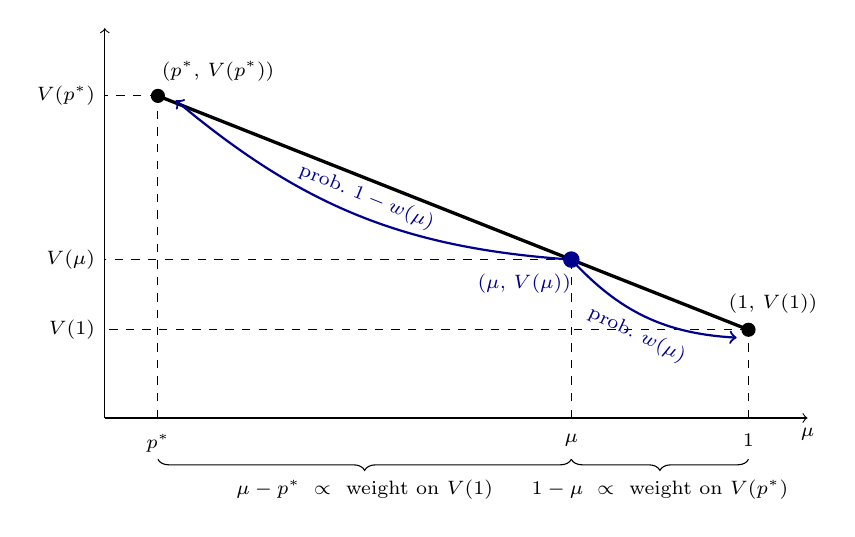
\begin{tikzpicture}[x=15cm, y=15cm, font=\scriptsize]
% axes (zoomed to the disclosure region)
\draw[->] (0.455,0.46) -- (1.05,0.46) node[below] {$\mu$};
\draw[->] (0.455,0.46) -- (0.455,0.79);
% chord and its endpoints
\draw[very thick] (0.5,0.7327) -- (1,0.5347);
\fill (0.5,0.7327) circle (0.006);
\fill (1,0.5347) circle (0.006);
\node[above right] at (0.495,0.737) {$(p^*,\,V(p^*))$};
\node[above right] at (0.975,0.540) {$(1,\,V(1))$};
% the interior point
\fill[blue!55!black] (0.85,0.5941) circle (0.007);
\node[below left, blue!55!black] at (0.858,0.590) {$(\mu,\,V(\mu))$};
% verticals and horizontals
\draw[dashed] (0.5,0.46) -- (0.5,0.7327);
\draw[dashed] (0.85,0.46) -- (0.85,0.5941);
\draw[dashed] (1,0.46) -- (1,0.5347);
\draw[dashed] (0.5,0.7327) -- (0.455,0.7327) node[left] {$V(p^*)$};
\draw[dashed] (0.85,0.5941) -- (0.455,0.5941) node[left] {$V(\mu)$};
\draw[dashed] (1,0.5347) -- (0.455,0.5347) node[left] {$V(1)$};
% axis ticks
\node[below] at (0.5,0.455) {$p^*$};
\node[below] at (0.85,0.455) {$\mu$};
\node[below] at (1,0.455) {$1$};
% the split lottery: arrows from the interior point to the two posteriors
\draw[->, thick, blue!55!black] (0.85,0.5941) to[bend left=18]
  node[midway, above, sloped] {prob.\ $1-w(\mu)$} (0.515,0.729);
\draw[->, thick, blue!55!black] (0.85,0.5941) to[bend right=22]
  node[midway, below, sloped] {prob.\ $w(\mu)$} (0.99,0.528);
% lever-rule braces under the axis
\draw[decorate, decoration={brace, mirror, amplitude=4pt}] (0.5,0.425) -- (0.85,0.425)
  node[midway, below=4pt] {$\mu-p^*\ \propto\ $ weight on $V(1)$};
\draw[decorate, decoration={brace, mirror, amplitude=4pt}] (0.85,0.425) -- (1,0.425)
  node[midway, below=4pt] {$1-\mu\ \propto\ $ weight on $V(p^*)$};
\end{tikzpicture}
\caption{The convex combination \eqref{eq:chord2} drawn geometrically, zoomed to the disclosure region $[p^*,1]$. The point $(\mu,V(\mu))$ on the chord is the barycenter of the endpoints $(p^*,V(p^*))$ and $(1,V(1))$ with weights $1-w(\mu)$ and $w(\mu)$; by the lever rule, each endpoint's weight is proportional to the distance from $\mu$ to the \emph{other} endpoint. The same two numbers reappear as the probabilities of the Bayes-plausible rationing split (blue arrows): with probability $w(\mu)$ the household is sent to posterior $1$ (\textsc{raise}) and with probability $1-w(\mu)$ to posterior $p^*$ (\textsc{cut} guidance), which is why evaluating the affine $V$ at $\mu$ and running the optimal split at $\mu$ are the same computation. Drawn for the same parameters as Figure~\ref{fig:geometry} at $\mu=1-b=0.85$ --- the binding belief of Section~\ref{Partial} --- where $w=0.7$ and $V(\mu)=0.3\cdot V(p^*)+0.7\cdot V(1)=0.594$.}
\label{fig:convexcomb}
\end{figure}

Now we may look at everything more closely and evaluate the function at $\mu=1$ and $\mu=p^*$. We know that $V\circ f(1) = V(f(1))$ where $f(1) = a+(1-a-b) = 1-b$. Similarly, according to the principal's payoff, $(1-\delta)u(1) = 0$. At the vertex $\mu=1$ the belief is degenerate --- all probability mass sits on $R$ --- and Bayes plausibility rules out any informative signal: a lottery over posteriors $\nu\in[0,1]$ with mean $\mathbb{E}_q[\nu]=1$ must place probability one on $\nu=1$, since an average of numbers no larger than $1$ equals $1$ only if every realization equals $1$. A household certain of a recession cannot be persuaded otherwise, so every policy at $\mu=1$ is outcome-equivalent to uninformative guidance, and the maximum in \eqref{eq:bellman} degenerates to a single plan: the bank receives the flow payoff $(1-\delta)u(1)=0$ in the current period, and the belief propagates to $f(1)=1-b$. With both terms known, and evaluating the chord \eqref{eq:chord2} at $\mu = 1-b \in (p^*,1)$, equation \eqref{eq:cav} gives:
\begin{equation}\label{eq:Beq}
V(1) = \delta V(1-b) = \delta\,\frac{b\,V(p^*) + (1-b-p^*)\,V(1)}{1-p^*}
\end{equation}
Taking similar steps at the threshold, where the household still spends so the flow is $(1-\delta)u(p^*) = 1-\delta$, and where uninformative guidance propagates the belief to
\[
\varphi := f(p^*) = a + (1-a-b)p^* \in (p^*, 1),
\]
we also obtain:
\begin{equation}\label{eq:Aeq}
V(p^*) = (1-\delta) + \delta V(\varphi)
= (1-\delta) + \delta\,\frac{(1-\varphi)\,V(p^*) + (\varphi-p^*)\,V(1)}{1-p^*},
\end{equation}
again using the chord \eqref{eq:chord2}, now at $\mu = \varphi$. Equations \eqref{eq:Beq} and \eqref{eq:Aeq} are two linear equations in the two unknowns $V(p^*)$ and $V(1)$; we now solve them explicitly.

\subsection{Solving the two-equation system}\label{Solving}

\paragraph{Step 1: solve \eqref{eq:Beq} for $V(1)$ in terms of $V(p^*)$.}
Multiply \eqref{eq:Beq} through by $1-p^*$ and collect the $V(1)$ terms:
\begin{align*}
(1-p^*)\,V(1) &= \delta b\,V(p^*) + \delta(1-b-p^*)\,V(1)\\
\big[(1-p^*) - \delta\big((1-p^*)-b\big)\big]V(1) &= \delta b\,V(p^*)\\
\big[(1-p^*)(1-\delta) + \delta b\big]V(1) &= \delta b\,V(p^*).
\end{align*}
Writing $q := 1-p^*$ and $\Delta := q(1-\delta) + \delta b > 0$,
\begin{equation}\label{eq:V1}
\boxed{\;V(1) = \frac{\delta b}{\Delta}\,V(p^*)\;},
\qquad \Delta = (1-p^*)(1-\delta) + \delta b .
\end{equation}

\paragraph{Step 2: substitute into \eqref{eq:Aeq} and solve for $V(p^*)$.}
Multiply \eqref{eq:Aeq} through by $q = 1-p^*$:
\[
q\,V(p^*) = (1-\delta)\,q + \delta(1-\varphi)\,V(p^*) + \delta(\varphi-p^*)\,V(1).
\]
Substituting \eqref{eq:V1} for $V(1)$,
\[
q\,V(p^*) - \delta(1-\varphi)\,V(p^*) - \frac{\delta^2 b\,(\varphi-p^*)}{\Delta}\,V(p^*) = (1-\delta)\,q,
\]
so that
\begin{equation}\label{eq:Vstar}
\boxed{\;V(p^*) = \frac{(1-\delta)(1-p^*)}{\,(1-p^*) - \delta(1-\varphi) - \dfrac{\delta^2 b\,(\varphi-p^*)}{\Delta}\,}\;},
\qquad \varphi - p^* = (a+b)(\mu_R^*-p^*) > 0 .
\end{equation}
Equations \eqref{eq:V1} and \eqref{eq:Vstar}, together with the chord \eqref{eq:chord2}, deliver $V$ in closed form on all of $[p^*,1]$.

\paragraph{Consistency checks.} Three checks confirm the solution is well behaved.
\emph{(i) The denominator of \eqref{eq:Vstar} is positive and $V(p^*)\le 1$.} Since $\Delta > \delta b$, the last term satisfies $\tfrac{\delta^2 b(\varphi-p^*)}{\Delta} < \delta(\varphi-p^*)$; hence
\[
(1-p^*) - \delta(1-\varphi) - \frac{\delta^2 b(\varphi-p^*)}{\Delta}
> (1-p^*) - \delta(1-\varphi) - \delta(\varphi-p^*)
= (1-p^*)(1-\delta) > 0,
\]
which simultaneously shows $V(p^*) < 1$: the bank cannot do better than the household spending in every period, whose normalized value is $1$.
\emph{(ii) $0 < V(1) < V(p^*)$.} Immediate from \eqref{eq:V1} since $0 < \tfrac{\delta b}{\Delta} < 1$; the value is higher at the threshold than at certainty of recession, as it must be, and $V$ is decreasing along the chord.
\emph{(iii) The absorbing limit recovers Ely.} As $b\to 0$ the recession never ends and we should recover Ely's absorbing beeps, where reaching certainty is terminal. Indeed $\Delta \to q(1-\delta) \ne 0$ while the numerator of \eqref{eq:V1} carries the factor $b\to 0$, so $V(1)\to 0$. For $b>0$ we have $V(1)>0$: reaching certainty of recession is no longer terminal, because the chain eventually leaves $R$ and the household resumes spending. This positive continuation value at the top of the simplex is the structural novelty of the recurrent chain, and it is exactly what the partial-commitment analysis of Section~\ref{Partial} leans on.

\paragraph{Interpretation of the two solutions.} Since the flow payoff is $1$ exactly when the household spends, $V(\mu)$ is the discounted fraction of future periods in which the household spends, starting from public belief $\mu$. The two solved values then read as follows. $V(p^*)$ is the value of the bank's ongoing operation at the obedience boundary --- the delay--ration--confess--recover cycle of Section~\ref{Policy}, measured at its rationing anchor, where the household is exactly indifferent. $V(1)$ is the value of the bank's future \emph{after telling the truth}: from the vertex the bank earns nothing today and waits for the drift, $V(1)=\delta V(1-b)$, so $V(1)$ is a pure recurrence premium --- the fraction $\delta b/\Delta$ of the threshold value that survives a confession. The pair suffices to describe the entire solution because the optimal policy only ever induces two posteriors, $p^*$ (keep spending) and $1$ (confession): the whole dynamic problem reduces to valuing these two destinations, and every other value in the disclosure region is their convex combination along the chord.

%--------------------------------------Policy---------------------------------
\section{Optimal disclosure policy}\label{Policy}

The optimal policy is read off the concave envelope in the manner of Ely (2017): issue uninformative guidance where the envelope coincides with the inner objective, and randomize (disclose) where the envelope strictly exceeds it. This gives a three-phase belief path.

\paragraph{Phase A --- uninformative guidance and upward drift ($\mu \le p^*$).} While the belief is below the threshold the bank issues uninformative \textsc{cut} guidance --- guidance uncorrelated with the state, in the sense defined in Section~\ref{Model} --- collecting the flow payoff $1$ each period while the belief drifts. Subtracting the fixed-point identity $\mu_R^* = a+(1-a-b)\mu_R^*$ from $\mu_{t+1} = a+(1-a-b)\mu_t$ and iterating from $\mu_0$,
\begin{equation}\label{eq:drift}
\mu_t = \mu_R^* + (1-a-b)^t\,(\mu_0 - \mu_R^*),
\end{equation}
so the belief converges monotonically toward $\mu_R^*$. Starting from $\mu_0 < p^* < \mu_R^*$, setting $\mu_{t^*} = p^*$ and solving,
\begin{equation}\label{eq:hit}
t^* = \frac{\ln\dfrac{\mu_R^*-p^*}{\mu_R^*-\mu_0}}{\ln(1-a-b)} > 0,
\end{equation}
and in discrete time the belief reaches or just crosses $p^*$ at the integer period $T(\mu_0) = \lceil t^* \rceil$. This is the recurrent analogue of the initial silent phase of Ely (2017): only the drift constant $1-a-b$ and the resting point $\mu_R^*$ have changed.

\paragraph{Phase B --- rationing at the threshold.} Once $\mu$ reaches $p^*$, the no-information drift would carry it to $f(p^*) = \varphi > p^*$, into the region where the household stops spending. To hold the belief on the threshold, the bank issues the informative \textsc{raise} \emph{only} in state $R$, at a rate $\rho \in [0,1]$, and never in state $N$; the residual message in either state is \textsc{cut} guidance. The single number $\rho$ is the \emph{disclosure rate}: $\rho=1$ is full confession, $\rho=0$ is stonewalling, and the \textsc{cut} sent in state $R$ (probability $1-\rho$) is a deliberate false negative. Two pressures pin $\rho$ down. The bank wants $\rho$ small, because every \textsc{raise} sends the posterior to $1$ and stops spending today; but the smaller is $\rho$, the more the \textsc{cut} message is contaminated by concealed recessions, and the household discounts the reassurance accordingly. The cheapest $\rho$ that preserves obedience therefore places the post-\textsc{cut} belief exactly on the boundary. After the drift the pre-disclosure belief is some $\mu > p^*$; conditioning on the event ``\textsc{cut} guidance'' and requiring the posterior to equal $p^*$:
\[
\Pr(R \mid \textsc{cut}) = \frac{\mu(1-\rho)}{\mu(1-\rho) + (1-\mu)\cdot 1} \stackrel{!}{=} p^* .
\]
Cross-multiplying and solving for $\rho$:
\begin{align*}
\mu(1-\rho) &= p^*\big[\mu(1-\rho) + (1-\mu)\big]\\
\mu(1-\rho)(1-p^*) &= p^*(1-\mu)\\
1-\rho = \frac{p^*(1-\mu)}{\mu(1-p^*)}
\;&\Longrightarrow\;
\rho = \frac{\mu(1-p^*) - p^*(1-\mu)}{\mu(1-p^*)} ,
\end{align*}
hence the threshold-holding disclosure rate is
\begin{equation}\label{eq:rhostar}
\boxed{\;\rho^*(\mu) = \frac{\mu - p^*}{\mu\,(1-p^*)}\;}
\end{equation}
This is the ``false-negative'' message that pins the belief on the obedience boundary: conditional on \textsc{cut} guidance, the household is just willing to keep spending --- the \textsc{cut} signal pools the two states in exactly the proportion that leaves the household indifferent. Three checks confirm the formula. First, $\rho^*(p^*)=0$: at the threshold itself no disclosure is needed yet. Second, $\rho^*(1)=1$: at certainty only full confession is consistent --- a mass point cannot be diluted, as in the vertex argument of Section~\ref{Bellman}. Third, the unconditional probability of a \textsc{raise} is $\mu\,\rho^*(\mu) = (\mu-p^*)/(1-p^*)$, precisely the weight $w(\mu)$ of \eqref{eq:weight} that the Bayes-plausible split places on the posterior $1$ (Figure~\ref{fig:convexcomb}): deriving $\rho^*$ from the household's conditional inference and reading the split off the concavification chord are the same computation. Finally, $\rho^*$ is increasing in $\mu$, which is what later selects the binding belief for credibility (Section~\ref{Partial}).

\paragraph{Phase C --- the recurrent cycle.} When \textsc{raise} is issued, the message reveals state $R$ (the rate is raised only in $R$), so the posterior jumps to $\mu = 1$. In Ely's absorbing model this would be terminal. In the recurrent chain it is not: from $\mu=1$ the drift pulls the belief back down through $f(1) = 1-b$ toward $\mu_R^*$, the belief re-enters the rationing region, and the cycle repeats. This is why $V(1)>0$ in \eqref{eq:V1}: the bank periodically gets the household expanding again.

\begin{prop}[Optimal full-commitment policy]\label{prop:optfc}
Under the non-degeneracy condition $p^* < \mu_R^*$, the optimal full-commitment policy is ``delay-then-ration'': issue uninformative guidance while $\mu \le p^*$ (Phase A), and once $\mu = p^*$ issue \textup{\textsc{raise}} only in state $R$, at the rate $\rho^*(\mu)$ in \eqref{eq:rhostar} that holds the post-\textup{\textsc{cut}} belief at $p^*$ (Phase B). Disclosure is non-terminal: after a \textup{\textsc{raise}} the belief drifts down from $1$ and the cycle repeats (Phase C).
\end{prop}

This answers the research question in the affirmative for the full-commitment case: the optimum does delay disclosure while recession risk is low, then reveals a state change only as often as obedience ($\mu \le p^*$) requires.

%--------------------------------------Partial commitment---------------------------------
\section{Partial commitment}\label{Partial}

We now relax commitment using the stochastic-commitment formulation of Min (2021) and Lipnowski, Ravid, and Shishkin (2022): each period the announced disclosure rule is honoured with probability $\lambda \in [0,1]$, and with probability $1-\lambda$ the bank re-optimises (cheats) given the current state. The question becomes when the delay-then-ration policy of Proposition~\ref{prop:optfc} survives period by period.

\paragraph{The credibility constraint.} The temptation to cheat is largest exactly when the bank is supposed to raise: a \textsc{raise} makes the household stop spending today, which is precisely the outcome the bank dislikes in the short run. (That the re-optimising bank always prefers the uninformative \textsc{cut} guidance is verified by a one-shot-deviation check with state-contingent continuation values; see Section~\ref{Progress}.) With honouring probability $\lambda$, the \emph{realised} \textsc{raise} rate in state $R$ is $\lambda\rho$ rather than the promised $\rho$. For the household to remain obedient --- to keep the post-\textsc{cut} belief at or below $p^*$ --- the realised disclosure must be at least the required rate at the relevant belief:
\[
\lambda\rho \;\ge\; \rho^*(\mu) \quad\text{at the on-path belief } \mu .
\]
Since the bank can promise at most $\rho = 1$ (\textsc{raise} with certainty in $R$), credibility requires $\lambda \ge \rho^*(\mu)$ at every on-path belief where rationing operates, hence at the \emph{largest} such belief.

\paragraph{The binding belief.} From \eqref{eq:rhostar}, $\partial\rho^*/\partial\mu = \tfrac{p^*}{\mu^2(1-p^*)} > 0$, so the worst case is the largest belief at which the bank still rations. After a \textsc{raise} the belief is $1$ and then drifts to $f(1) = 1-b$; this is the highest pre-disclosure belief the rationing phase must contend with on the cycle. Evaluating \eqref{eq:rhostar} there gives the dynamic commitment threshold.

\begin{prop}[Sustainability of persuasion]\label{prop:lambda}
The delay-then-ration policy is sustainable under partial commitment if and only if the honouring probability satisfies
\begin{equation}\label{eq:lambda}
\boxed{\;\lambda \;\ge\; \lambda_{\mathrm{dyn}} := \rho^*(1-b) = \frac{1-b-p^*}{(1-b)(1-p^*)}\;}
\end{equation}
\end{prop}

The threshold is well posed because $p^* < \mu_R^* < 1-b$ (the latter since $\tfrac{a}{a+b} \le 1-b \iff 0 \le b(1-a-b)$).

\paragraph{Comparative statics.} Write $c := 1-b$, so $\lambda_{\mathrm{dyn}} = \tfrac{c-p^*}{c(1-p^*)}$. Differentiating with respect to the threshold,
\[
\frac{\partial\lambda_{\mathrm{dyn}}}{\partial p^*}
= \frac{-c(1-p^*) + (c-p^*)\,c}{c^2(1-p^*)^2}
= \frac{c-1}{c(1-p^*)^2}
= \frac{-b}{(1-b)(1-p^*)^2} < 0 :
\]
a more lenient household (larger $p^*$) lowers the commitment needed. Rewriting $\lambda_{\mathrm{dyn}} = \tfrac{1}{1-p^*} - \tfrac{p^*}{(1-p^*)(1-b)}$ and differentiating with respect to the exit rate,
\[
\frac{\partial\lambda_{\mathrm{dyn}}}{\partial b}
= -\frac{p^*}{1-p^*}\cdot\frac{d}{db}\Big(\frac{1}{1-b}\Big)
= -\frac{p^*}{(1-p^*)(1-b)^2} < 0 :
\]
a more persistent recession (smaller $b$) \emph{raises} the required commitment. In the limits: $b\to 0$ gives $\lambda_{\mathrm{dyn}} \to 1$ (permanent recessions demand full commitment, recovering the absorbing benchmark), while $b \uparrow 1-p^*$ gives $\lambda_{\mathrm{dyn}} \to 0$. Note that $b\to 0$ is exactly the limit in which $V(1)\to 0$ (Section~\ref{Solving}): the positive continuation value at the top of the simplex and the sufficiency of \emph{partial} commitment are the same phenomenon viewed from the value side and the constraint side. The following theorem records the equivalence formally.

\begin{thm}[Recurrence, positive continuation value, and partial commitment]\label{thm:equiv}
Fix $a\in(0,1)$, $\delta\in(0,1)$, and the non-degeneracy condition $p^*<\mu_R^*$, and allow $b\in[0,1-a)$. The following statements are equivalent:
\begin{enumerate}
\item[(i)] $b>0$;
\item[(ii)] $f(1)<1$: certainty of recession is not a fixed point of the belief map;
\item[(iii)] the state chain $P$ is irreducible, hence ergodic;
\item[(iv)] $V(1)>0$;
\item[(v)] $\lambda_{\mathrm{dyn}}<1$.
\end{enumerate}
At $b=0$ all five fail simultaneously: $R$ is absorbing, $V(1)=0$, and $\lambda_{\mathrm{dyn}}=1$, recovering the benchmark of Ely (2017), where only full commitment sustains disclosure.
\end{thm}

\begin{pf}
\emph{(i) $\Leftrightarrow$ (ii).} Direct computation: $f(1)=a+(1-a-b)=1-b$, so $f(1)<1$ if and only if $b>0$.

\emph{(i) $\Leftrightarrow$ (iii).} A finite chain is irreducible if and only if all states communicate. Since $a>0$ is maintained, both off-diagonal entries of $P$ are positive if and only if $b>0$; an irreducible finite chain is positive recurrent with the unique stationary distribution $\pi=(\tfrac{b}{a+b},\tfrac{a}{a+b})$, and the exit time from $R$ is geometric with mean $1/b<\infty$. Conversely, at $b=0$ the state $R$ is absorbing and $P$ is reducible.

\emph{(i) $\Leftrightarrow$ (iv).} The vertex equation \eqref{eq:Beq} reads $V(1)=\delta V(f(1))=\delta V(1-b)$. If $b=0$ this becomes $V(1)=\delta V(1)$, i.e.\ $(1-\delta)V(1)=0$, whose unique solution is $V(1)=0$ since $\delta<1$: the terminal condition of the absorbing model is forced, not assumed. If $b>0$, the solved system \eqref{eq:V1} gives $V(1)=\tfrac{\delta b}{\Delta}V(p^*)$ with $\Delta=(1-p^*)(1-\delta)+\delta b>0$, and $V(p^*)>0$ because its numerator $(1-\delta)(1-p^*)$ and denominator are both strictly positive (consistency check (i) of Section~\ref{Solving}). Hence $V(1)>0$ if and only if $b>0$.

\emph{(i) $\Leftrightarrow$ (v).} The rationing rate \eqref{eq:rhostar} is strictly increasing on $[p^*,1]$, with $\partial\rho^*/\partial\mu=p^*/(\mu^2(1-p^*))>0$ and $\rho^*(1)=\tfrac{1-p^*}{1\cdot(1-p^*)}=1$. Since $\lambda_{\mathrm{dyn}}=\rho^*(1-b)$, direct algebra gives
\[
1-\lambda_{\mathrm{dyn}}
=\frac{(1-b)(1-p^*)-(1-b-p^*)}{(1-b)(1-p^*)}
=\frac{b\,p^*}{(1-b)(1-p^*)},
\]
which is strictly positive if and only if $b>0$.
\end{pf}

The last display quantifies the link: both the continuation value at the top of the simplex, $V(1)=\tfrac{\delta b}{\Delta}V(p^*)$, and the commitment slack, $1-\lambda_{\mathrm{dyn}}=\tfrac{b\,p^*}{(1-b)(1-p^*)}$, vanish \emph{linearly} in $b$. Recurrence is therefore not qualitative background: $b$ is the common small parameter governing simultaneously how much future the bank retains after a confessed recession and how much credibility it is allowed to lack.

\begin{prop}[Persistence, not arrival, drives the commitment need]\label{prop:speed}
$\lambda_{\mathrm{dyn}}$ is independent of the onset rate $a$, strictly decreasing in the threshold $p^*$, and strictly decreasing in the exit rate $b$. Equivalently, the commitment requirement is governed by the expected recession duration $1/b$: longer-lasting recessions demand more commitment, while how often recessions arrive is irrelevant.
\end{prop}

%--------------------------------------Progress and next steps---------------------------------
\section{Progress summary and next steps}\label{Progress}

Relative to the last report, the full-commitment benchmark is now solved in closed form (equations \eqref{eq:V1} and \eqref{eq:Vstar}), the optimal policy is characterized (Proposition~\ref{prop:optfc}), and the partial-commitment layer delivers a single sufficient statistic $\lambda_{\mathrm{dyn}}$ for whether persuasion is sustainable (Proposition~\ref{prop:lambda}), driven by recession \emph{persistence} rather than \emph{incidence} (Proposition~\ref{prop:speed}).

In the working draft the credibility argument has additionally been closed with a formal one-shot-deviation check (Mailath \& Samuelson 2006). Because the bank observes the true state while $V$ tracks only the public belief, the check requires \emph{state-contingent} continuation values; the on-path rationing beliefs form the finite cycle $\{\varphi, 1-b\}$, so these values solve a small linear system, and the free bank's gain from suppressing the \textsc{raise} is $(1-\delta)/(1-\theta) > 0$ with $\theta := \delta(1-b)\big[\rho^*(1-b) - \rho^*(\varphi)\big]$ --- strictly positive everywhere, confirming that a cheating bank always issues the uninformative \textsc{cut} guidance and that \eqref{eq:lambda} is an if-and-only-if. A further outcome-equivalence result shows the bank's value is \emph{flat} in $\lambda$ above $\lambda_{\mathrm{dyn}}$: all the economics of partial commitment is concentrated in the cutoff.

Three extensions remain for the final report. First, \emph{endogenous commitment}: here $\lambda$ is exogenous (Min 2021); the goal stated in the research question is to make it an equilibrium object, e.g.\ a reputation state updated after observed cheats as in Best \& Quigley (2024). Second, \emph{behavior below the cutoff}: characterizing the optimal (necessarily coarser) disclosure when $\lambda < \lambda_{\mathrm{dyn}}$. Third, \emph{the FX welfare channel}: the exchange-rate externality of the Introduction has not yet entered the payoff; folding it in would let the model speak to the trade-off between domestic consumption smoothing and the export subsidy implicit in a deflated currency.

%--------------------------------------References---------------------------------
\newpage
\begin{thebibliography}{99}

\bibitem{as2025} Arieli, I. and Stewart, C. (2025). Bayesian Persuasion without Commitment. Working paper, arXiv:2511.18662.

\bibitem{bq2024} Best, J. and Quigley, D. (2024). Persuasion for the Long Run.

\bibitem{cs1982} Crawford, V. and Sobel, J. (1982). Strategic Information Transmission. \textit{Econometrica} 50(6), 1431--1451.

\bibitem{dlm2018a} Danilov, V. I. and Lambert-Mogiliansky, A. (2018a). Targeting in Quantum Persuasion Problem. \textit{Journal of Mathematical Economics} 78, 142--149.

\bibitem{dlm2018b} Danilov, V. I. and Lambert-Mogiliansky, A. (2018b). Preparing a (Quantum) Belief System. \textit{Theoretical Computer Science} 752, 97--103.

\bibitem{ely2017} Ely, J. (2017). Beeps. \textit{American Economic Review} 107(1), 31--53.

\bibitem{kg2011} Kamenica, E. and Gentzkow, M. (2011). Bayesian Persuasion. \textit{American Economic Review} 101(6), 2590--2615.

\bibitem{lrs2022} Lipnowski, E., Ravid, D., and Shishkin, D. (2022). Persuasion via Weak Institutions. \textit{Journal of Political Economy} 130(10), 2705--2730.

\bibitem{ms2006} Mailath, G. and Samuelson, L. (2006). \textit{Repeated Games and Reputations: Long-Run Relationships}. Oxford University Press.

\bibitem{min2021} Min, D. (2021). Bayesian Persuasion under Partial Commitment. \textit{Economic Theory}.

\bibitem{spence1973} Spence, M. (1973). Job Market Signaling. \textit{Quarterly Journal of Economics} 87(3), 355--374.

\end{thebibliography}

\end{document}
